\documentclass[12pt, a4paper]{article}
\usepackage{bm, float,amsmath,graphicx}
\graphicspath{ {./images/} }
\usepackage[T1]{fontenc}
\usepackage[polish]{babel}
\usepackage[utf8]{inputenc}

\title{Metody optymalizacji}
\author{Stepan Yurtsiv, 246437}
\date{9 maja 2022r.}

\begin{document}
\maketitle

\section{Zadanie 1}

Celem danego zadania jest wyznaczenie serwerów, z których należy odczytać dane o określonych cechach,
aby zminimalizować czas.

\subsection{Model}

\textbf{Funkcja celu:}

\begin{center}
	min \textbf{$\displaystyle\sum_{j \in [n]} x_j * T_j$}
\end{center}
gdzie

\begin{itemize}
    \item $n$ - liczba serwerów
    \item $T_j$ - czas odczytu danych z serwera $j \in [n]$
    \item $x_j$ - zmienna binarna określająca, czy serwer $j$ powinien zostać przeszukany, $x_j \in \{0, 1\}$, $j \in [n]$
\end{itemize}
\textbf{Ograniczenia:}

\begin{itemize}
    \item {$\forall{i \in [m]}\displaystyle\sum_{j \in [n]} Q_{ij} * x_j \geq 1$}, gdzie $m$ - liczba cech, a $Q_{ij}$ określa, czy dane cechy $i$ są na serwerze $j$. Dane ograniczenie zapewnia, że dane każdej cechy zostaną przeczytane co najmniej raz.
\end{itemize}

\subsection{Wyniki}

Zdefiniowano następujący egzemplarz problemu

\begin{table}[H]
\begin{center}
\begin{tabular}{|c|c|}
  \hline
  Serwer & Czas \\
  \hline
  1 & 4 \\
  \hline
  2 & 2 \\
  \hline
  3 & 5 \\
  \hline
  4 & 1 \\
  \hline
  5 & 6 \\
  \hline
\end{tabular}
\caption{Czas odczytu danych dla każdego serwera}
\end{center}
\end{table}

\begin{table}[H]
\begin{center}
\begin{tabular}{|c|c|c|c|c|c|}
  \hline
  Cecha / Serwer & 1 & 2 & 3 & 4 & 5 \\
  \hline
  1 & 0 & 0 & 0 & 0 & 1 \\
  \hline
  2 & 1 & 1 & 1 & 1 & 0 \\
  \hline
  3 & 1 & 0 & 0 & 1 & 0 \\
  \hline
  4 & 0 & 1 & 1 & 1 & 0 \\
  \hline
  5 & 1 & 0 & 0 & 0 & 0 \\
  \hline
  6 & 0 & 0 & 0 & 1 & 0 \\
  \hline
  7 & 0 & 0 & 1 & 1 & 0 \\
  \hline
\end{tabular}
\caption{Obecność danych cech na każdym serwerze}
\end{center}
\end{table}

Dla tych danych optymalnym rozwiązaniem jest pobranie danych z serwerów 1, 4 i 5. Sumaryczny czas wyniesie 11 jednostek.

 
\section{Zadanie 2}

Zadanie 2 polega na ułożeniu sekwencyjnego programu, skaładającego się z określonego zbioru funkcji $I$. Należy
dobrać odpowiednie podprogramy, aby cały program zajmował nie więcej niż $M$ komórek pamięci, a czas jego wykonaia był minimalny.


\subsection{Model}

\textbf{Funkcja celu:}

\begin{center}
	min \textbf{$\displaystyle\sum_{i \in I, j \in [m]} x_{ij} * T_{ij}$}
\end{center}
gdzie

\begin{itemize}
    \item $m$ - liczba podprogramów do obliczenia funkcji
    \item $I$ - zbiór funkcji do policzenia. $i \in I \leq n$, gdzie $n$ to liczba wszystkich możliwych funkcji
    \item $T_{ij}$ - czas działania podgprogramu $j$ dla funkcji $i$
    \item $x_{ij}$ - zmienna binarna określająca, czy podprogram $j$ zostanie użyty do policzenia funkcji $i$. $x_{ij} \in \{0, 1\}$, $i \in I$, $j \in [m]$
\end{itemize}
\textbf{Ograniczenia:}

\begin{itemize}
    \item {$\displaystyle\sum_{i \in I, j \in [m]} x_{ij} * R_{ij} \leq M$}, gdzie $R_{ij}$ to ilość pamięci, wymagana przez podprogram $j$. Dane ograniczenie zapewnia, że cały program zużywa maksymalnie $M$ komórek pamięci
    \item {$\forall{i \in I}\displaystyle\sum_{j \in [m]} x_{ij} = 1$} - zapewnia wybranie dokładnie jednego podgprogramu dla danej funkcji
\end{itemize}

\subsection{Wyniki}

Zdefiniowano następujący egzemplarz problemu:
$I = \{1, 2, 4\}$, $M = 15$

\begin{table}[H]
\begin{center}
\begin{tabular}{|c|c|c|c|c|}
  \hline
  Funkcja / Podprogram & 1 & 2 & 3 & 4 \\
  \hline
  1 & 3 & 2 & 1 & 9 \\
  \hline
  2 & 1 & 2 & 3 & 5 \\
  \hline
  3 & 4 & 5 & 2 & 8 \\
  \hline
  4 & 1 & 8 & 2 & 8 \\
  \hline
\end{tabular} 
\caption{Wymgania pamięciowe}
\end{center}
\end{table}

\begin{table}[H]
\begin{center}
\begin{tabular}{|c|c|c|c|c|}
  \hline
  Funkcja / Podprogram & 1 & 2 & 3 & 4 \\
  \hline
  1 & 4 & 6 & 9 & 2 \\
  \hline
  2 & 10 & 8 & 7 & 5 \\
  \hline
  3 & 3 & 5 & 2 & 1 \\
  \hline
  4 & 15 & 2 & 8 & 3 \\
  \hline
\end{tabular} 
\caption{Wymagania czasowe}
\end{center}
\end{table}

Otrzymano następujące rozwiązanie optymalne:

\begin{itemize}
    \item Czas wykonania programu: 13
    \item Zużycie pamięci: 15
\end{itemize}

\begin{table}[H]
\begin{center}
\begin{tabular}{|c|c|c|c|c|}
  \hline
  Funkcja / Podprogram & 1 & 2 & 3 & 4 \\
  \hline
  1 & & x & &  \\
  \hline
  2 &  &  & & x \\
  \hline
  4 &  & x &  &  \\
  \hline
\end{tabular} 
\caption{Których podprogramów użyć}
\end{center}
\end{table}

\section{Zadanie 3}

Dane zadanie polega na stworzeniu harmonogramu wynonania zdań na procesorach.

\subsection{Model}

Niech:
\begin{itemize}
    \item $n$ - liczba procesorów
    \item $m$ - liczba zadań do wykonania
    \item $T_{ji}$ - czas wykonania zadania $j$ na procesorze $i$
    \item $O_{jik}$ - zmienna pomocnicza binarna, wyznaczająca kolejność zadań. $O_{jik} = 1$ ozanacza że zadanie $i$ zaczyna się szybciej od zadania $k$ na procesorze $j$
    \item $S_{ji}$ - czas rozpoczęcia zadania $i$ na procesorze $j$
    \item $C_{max}$ - czas zakończenia wszystkich zadań
    
\end{itemize}

\subsubsection*{Funkcja celu:}

\begin{center}
	min $C_{max}$
\end{center}

\subsubsection*{Ograniczenia:}

\begin{itemize}
    \item Wsyzstkie zadania muszą być zakończone przed zakończenim ostatniego
    \begin{center}
    	$\forall{(i \in [m])} S_{ni} + T_{ni} \leq C_{max}$
    \end{center}

    \item Każdy procesor może wykonywać tylko jedno zadania naraz
        \begin{center}
        	$\forall{(j \in [n], i, k \in [m])} S_{jk} \geq S_{ji} + T_{ji} $
            , jeżeli 
            $ O_{jik} = 1 $
        	$\forall{(j \in [n], i, k \in [m])} S_{ji} \geq S_{jk} + T_{jk} $
        	, jeżeli 
        	$ O_{jik} = 0 $ \\ 
        \end{center}
    \item Wykonanie zadania może się zacząć tylko po jego zakończeniu na poprzednim procesorze
    \begin{center}
    	$\forall{(i \in [m], j \in [n - 1])} S_{(j + 1)i} \geq S_{ji} + T_{ji} $
    \end{center}
    
\end{itemize}

\subsection{Wyniki}

Zdefiniowano następujący egzemplarz problemu: $n = 3$

\begin{table}[H]
\begin{center}
\begin{tabular}{|c|c|c|c|c|}
  \hline
  Procesor / Zadanie & 1 & 2 & 3 & 4 \\
  \hline
  1 & 1 & 2 & 4 & 4 \\
  \hline
  2 & 3 & 1 & 2 & 4 \\
  \hline
  3 & 4 & 2 & 1 & 3 \\
  \hline
\end{tabular} 
\caption{Czas wykonania zadań na każdmy z procesorów}
\end{center}
\end{table}

Optymalnym jest następujący harmonogram:

\begin{figure}[H]
  \begin{center}
  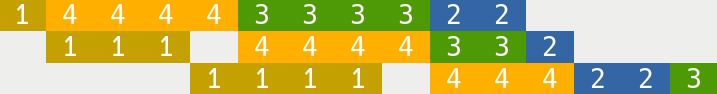
\includegraphics[scale=0.5]{Gantt}
  \end{center}
\end{figure}

$C_{max} = 15$

\end{document}

